%%%%%%%%%%%%%%%%%%%%%%%%%%%%%%%%%%%%%%%%%
% Journal Article
% LaTeX Template
% Version 1.4 (15/5/16)
%
% This template has been downloaded from:
% http://www.LaTeXTemplates.com
%
% Original author:
% Frits Wenneker (http://www.howtotex.com) with extensive modifications by
% Vel (vel@LaTeXTemplates.com)
%
% License:
% CC BY-NC-SA 3.0 (http://creativecommons.org/licenses/by-nc-sa/3.0/)
%
%%%%%%%%%%%%%%%%%%%%%%%%%%%%%%%%%%%%%%%%%

%----------------------------------------------------------------------------------------
%	PACKAGES AND OTHER DOCUMENT CONFIGURATIONS
%----------------------------------------------------------------------------------------

%\documentclass[twoside,twocolumn]{article}  
\documentclass[twoside]{article}  
\usepackage{amsmath}
\usepackage{relsize}
\usepackage{blindtext} % Package to generate dummy text throughout this template 
\usepackage{url}
\usepackage{hyperref}
\usepackage{indentfirst}

\usepackage[sc]{mathpazo} % Use the Palatino font
\usepackage[T1]{fontenc} % Use 8-bit encoding that has 256 glyphs
%\linespread{1.05} % Line spacing - Palatino needs more space between lines
\linespread{1.5} % Line spacing - Palatino needs more space between lines
\usepackage{microtype} % Slightly tweak font spacing for aesthetics

\usepackage[english]{babel} % Language hyphenation and typographical rules

\usepackage[hmarginratio=1:1,top=32mm,columnsep=20pt]{geometry} % Document margins
\usepackage[hang, small,labelfont=bf,up,textfont=it,up]{caption} % Custom captions under/above floats in tables or figures
\usepackage{booktabs} % Horizontal rules in tables

\usepackage{lettrine} % The lettrine is the first enlarged letter at the beginning of the text

\usepackage{enumitem} % Customized lists
\setlist[itemize]{noitemsep} % Make itemize lists more compact

\usepackage{abstract} % Allows abstract customization
\renewcommand{\abstractnamefont}{\normalfont\bfseries} % Set the "Abstract" text to bold
\renewcommand{\abstracttextfont}{\normalfont\small\itshape} % Set the abstract itself to small italic text

\usepackage{titlesec} % Allows customization of titles
%\renewcommand\thesection{\Roman{section}} % Roman numerals for the sections
%\renewcommand\thesubsection{\roman{subsection}} % roman numerals for subsections
\titleformat{\section}[block]{\large\scshape\centering}{\thesection.}{1em}{} % Change the look of the section titles
\titleformat{\subsection}[block]{\large}{\thesubsection.}{1em}{} % Change the look of the section titles

\usepackage{fancyhdr} % Headers and footers
\pagestyle{fancy} % All pages have headers and footers
\fancyhead{} % Blank out the default header
\fancyfoot{} % Blank out the default footer
\fancyhead[C]{Tokenized Services using SFTs $\bullet$  Feb. 2022} % Custom header text $\bullet$ Vol. XXI, No. 1
\fancyfoot[RO,LE]{\thepage} % Custom footer text
\usepackage{natbib}
\usepackage{titling} % Customizing the title section
\usepackage{listings}

%\usepackage[shortlabels]{enumitem}



\usepackage{hyperref} % For hyperlinks in the PDF
\usepackage{graphicx}
\graphicspath{ {./images/} }
\usepackage{caption}
\usepackage{subcaption}
 \usepackage{setspace}
%----------------------------------------------------------------------------------------
%	TITLE SECTION
%----------------------------------------------------------------------------------------
\setcitestyle{square}
\setlength{\droptitle}{-4\baselineskip} % Move the title up

\pretitle{\begin{center}\Large\bfseries} % Article title formatting
\posttitle{\end{center}} % Article title closing formatting
\title{Tokenized Time and Services Service Credits} % Article title
\author{%
\normalsize (Patent pending)\\ % Your institution
\\
\textsc{Joseph Egbulefu}\thanks{Founder at Meritic, www.meritic.xyz} \\[1ex] % Your name
\normalsize Meritic\\ % Your institution
\normalsize \href{mailto:joseph@meritic.xyz}{joseph@meritic.xyz} % Your email address
%\and % Uncomment if 2 authors are required, duplicate these 4 lines if more
%\textsc{Jane Smith}\thanks{Corresponding author} \\[1ex] % Second author's name
%\normalsize University of Utah \\ % Second author's institution
%\normalsize \href{mailto:jane@smith.com}{jane@smith.com} % Second author's email address
}
\date{July 31, 2023  \footnote{Version 1.0 of this document was published on October 16, 2022}} 
\renewcommand{\maketitlehookd}{%
\begin{abstract}
\noindent 

\end{abstract}
}







%----------------------------------------------------------------------------------------

\begin{document}

% Print the title
\maketitle

%----------------------------------------------------------------------------------------
%	ARTICLE CONTENTS
%----------------------------------------------------------------------------------------

\section{Introduction}
%\lettrine[nindent=0em,lines=3]{S}
\indent 

Web3 markets offer  several comparative advantages over their Web2 counterparts: provenance, smart-contract programmability, and decentralized secondary markets. Thus far though, many projects on Web3 marketplaces have, arguably, not significantly benefited from all three advantages.  A majority of digital assets belong to one of four categories: Works of Art (including Music), Virtual Gaming, Memberships and Event tickets, and Physical products. 
One cannot make similar arguments for Digital Art. Digital art collections have actually not benefited from provenance: due to  efficacy of LLMs in digital art, successful art collections will continue to contend with copy-cat collections in the market [Reference: https://www.plagiarismtoday.com/2023/06/28/yet-another-nft-plagiarism-scandal/]. This reality, coupled with the fact that art is traditionally illiquid suggests that secondary market activity for Digital Art is unlikely to grow significantly should the market recover. For physical goods, especially high-end fashion products, some brands are using the  blockchain to prevent fraud from imitation; however, most handbag or shoe owners are unlikely to resell or trade these items on the secondary market. Projects would derive more value from Web3 by tokenizing their time or service credits.credits.

\section{A case for credits}
Artwork and products are non-fungible. But credit is semi-fungible; and fungibility yields more options. In normal market conditions,  a credit holder has similar options as one holding the product, plus the option of redeeming the credit for said product, or waiting for the future when prices or offerings improve. For the creator or project, credits provide an efficient means to earn off-collection revenue: a prospect or follower may wish to incorporate a project’s creative elements  into her own work, rather than owning items in the existing  collection; a group of fans may prefer experiencing a private virtual one-on-one with a music artist, over owning his  tracks. 

For projects  with large followership or user base, service  credits offer higher potential for secondary market transactions, higher revenue potential via redemptions, and can better leverage programmability to implement credit expirations and transfer restrictions in code. And for provenance, it is straightforward to verify the service provider or merchant used credits from an authorized  sourcing or AI service, for instance. 

\section{Leveraging ERC-3525: The Semi-Fungible Token standard}
Projects  have not embraced credit issuance primarily because of infrastructural challenges: a lack of flexible SFT smart contract standards, and user friendly contract deployment process for issuing credits, and flexible redemption process. Until 2017 many projects minted their own ERC-20 fungible tokens, which served as funding vehicles and a form of credit since, in many cases, one had to acquire the tokens to access project offerings.  In late 2017 though, regulators curtailed that practice due to fraud associated with ICOs. Since then, Web3 projects  have relied on the ERC-721, the Non-fungible Token standard, and its successor, ERC-1155. While ERC-1155 can represent  fungibility  and non-fungibility alike, it does so by binding fungible value to wallet address rather than to token IDs, making it unsuitable for representing a semi fungible token.

ERC-3525, a new Ethereum semi-fungible token standard ratified in December 2022 is ideal for representing service credit. Each ERC-3525 token has a Token  ID, a Value, and a Slot ID. A creator or project will likely have offerings that differ by time, venue (virtual vs physical), coverage  or other features; each token ID associates to an offering issued to a customer. The value tracks how much credit is available on the token. As with an NFT, a holder of a 3525 token may sell / transfer  the token to another person; unlike NFTs, 3525 tokens enables the holder to transfer value from their token to another token with the same slot ID. For instance, you may have a special promotional or charity offering which you do not want to honor existing credit redemptions; then you would assign the promotional tokens to a new slot ID. 

Meritic’ has leveraged smart contract programmability to design four types of ERC-3525 service tokens.  
\begin{itemize}
\item Time credit: value represents units of time
\item Monetary credit: value represents monetary equivalent that is redeemable for purchases.
\item Items credit: holds a count of a specific offering or product 
\item Priority credit: value represents position in a waitlist or queue.
\end{itemize}

Traditionally merchant service credit is facilitated through gift or pre-paid cards: a customer pays an amount of money to the merchant or card network provider. That money is held in a bank account and a card with equivalent monetary value is issued to the customer. At some point in the future,  the customer uses the card to pay for service, the transaction value is transferred from the linked account to the merchant account and credit balance on the card is updated. If it is an open loop card then the customer can spend it in the credit with any merchant on the network, while in a closed loop, the customer can only redeem the credit at the merchant that issued the credit. Important features to replicate: the credit value is linked to real value which the merchant does not access until service is delivered to the customer. 

In our implementation, the creator / project configures then deploys an ERC-3525  smart contract for their service to the Polygon blockchain. The creator also creates a revenue wallet so that when token holders redeem token value for service, token underlying values are transferred to the creators revenue wallet  on the blockchain. The creator also lists a token collection to a Web3 marketplace where users can bid for or purchase the creators tokens.  Before we look at an example transaction, note that the value held in a service token may be backed by an underlying real value. This value is in USDC or ETH. In the example that follows we use USDC as the underlying. 

Figure \ref{schema} illustrates how funds flow to complete a service token primary sale.  First, a customer, Jack, purchase a token (Token #3 in the diagram) with a minimum bid price of 100 USDC. The customer pays the bid price plus commission to the marketplace.  The customer signs this transaction, giving approval for the USDC smart contract to transfer his funds to Meritic's marketplace wallet. In Step 2, Meritic deducts its commission and transfers the funds to Meritic's Wrapped USDC  contract. This contract facilitates pooling of token underlying values for each service contract. Next, Meritic sends a request to the creator's service contract, contract XYZ,  to mint Token #3 with value 100 and set Jack as owner.  The service contract starts the minting, which requires it to ask the Wrapped USDC contract to allocate an equivalent amount of underlying value to XYZ's underlying pool.  In Step 5, the Wrapped USDC contract  transfers 100, which it received from Meritic's marketplace wallet, to XYZ's USDC pool. Once this completes then Step 6, which requires XYZ contract to mark Jack as owner of Token #3, concludes the sale transaction. It is important to note that each service contract address holds its own token-holders underlying USDC in a pool. Whenever a Jack spend's a portion of his token value, underlying value is deducted from XYZ's pool and transferred to the creators revenue wallet. 



\begin{figure}[ht!]
     \centering
     \label{schema}
      \caption{Schematic of primary and secondary transactions. In a primary sale, the buyer takes ownership of the Service NFT from the subscription provider. In a secondary sale the buyer takes ownership from a previous buyer. }
         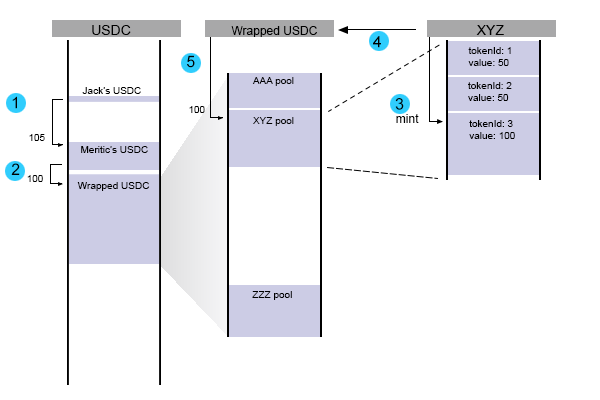
\includegraphics[scale=0.75]{tokenized_credit_explainer.png}
\end{figure}



\section{Credit at discount}
A project may issue credit at discount by, for example,  requiring a minimum bid of 70 USDC to own a token with 100 USDC of credit. Meritic’s implementation each token is minted  with a discount factor (in basis points), which is stored in the contract. When the customer redeems a partition of value for service, X units of credits then 

\begin{equation}
Y=(1-d)X\hspace{3pt} \text{USDC}
\end{equation}
Is released from the contract underlying  pool and transferred to the project’s receivables address. 
\subsection{Secondary market transactions}
A token holder conducts a secondary  market transaction when he sells his token  to another party in exchange for crypto currency  or other token  (a token swap). Such transactions may occur on centralized marketplaces,  decentralized exchanges such as Sudoswap,  or peer to peer wallet transfers.  For such transactions, the only change that occurs is the smart contract updates the token owner address with the wallet address of the new token holder. The token ID, Slot ID, and credit value remains unchanged; though the credit value of the token (should) inform the secondary market selling price for the token, the resulting selling price does not affect the credit value in the token 

As mentioned earlier, ERC-3525 introduced a new transfer mode: token-to-token value transfer for tokens with the same slot id. The token holder transfers a fraction of their credit value to another token (that may or may not be owned by someone else). When credits are transferred between tokens, the contract underlying value pool remains unchanged. However we must consider  the possibility that the two tokens have different discount factors, in which case the discount factor of the destination token must be updated. If the source token, with discount factor $d_s$, is transferring x units of credit to the destination token, with discount $d_d$  and y units of credit before transfer, then after value transfer the destination token has discount factor of 
\begin{equation}
d = 1 - \frac{(1-d_s)X +(1 - d_d)Y}{(X + Y)}
\end{equation}
For such value transfers, Meritic requires that the credit values be of the same type (monetary credit value cannot be transferred to time credit value).  

\section{Time Credit}
The smart contract requires a specified unit of time (hours, days, months, etc). However, all time tokens store credit value in seconds. Consider a primary token sale where  a customer pays 100 USDC for 1 hour of service time. As previously explained, the USDC value is locked in a Wrapped USDC owned by the project smart contract. Time credit contracts do not use discount factors. Instead, when a token is minted, the smart contract calculates the per-second time-value rate using the  primary sell price (100 USDC) and the time credit value (1 hour). If the token is given out for free then the time-value rate is zero. 

Time redemption occurs when the holder uses the service for some amount of time X (converted to seconds)  available on the token. A commensurate USDC value:
\begin{equation}
Y = sX
\end{equation}
 is released  from the contract’s USDC pool and transferred to the project's receivables address. 

As in the case of monetary credit, if the token owner conducts a secondary transaction that requires transferring the token to a new owner then smart-contract updates the token’s owner address while keeping the time-value rate and other token properties unchanged.  
When a token receives time-credit value via token-to-token value transfer then it is the credit destination and the other token is the credit source. In such a case, the smart contract must consider  the time-value rate $r_s$, of the  source token and update the rate, $r_d$,  of the destination token if, necessary. After value transfer, $r_d$, becomes:
\begin{equation}
r_d = \frac{r_sX + r_d Y}{X + Y}
\end{equation}

\end{document}
